% Proxies stand in for multiple versions, intercept all access, and forward to the correct version.


\chapter{Implementation} \label{chapter:IMPLEMENTATION}

This chapter describes how we used the ECMAScript 6 proxies\footnote{\url{http://wiki.ecmascript.org/doku.php?id=harmony:direct_proxies}, accessed February 3rd, 2014} to implement version-aware references for the Lively Kernel.
It presents the proxy's behavior and shows how proxies are inserted for ordinary references using source transformations.
The chapter also presents implemented workarounds for the current state of ECMAScript 6 proxies.
It concludes with current limitations.

\section{ECMAScript 6 Proxies as Version-aware References} \label{sec:IMPLEMENTATION:1}

This section first describes the proxies proposed with the next version of JavaScript's standard~\cite{Ecma2014ES6}.
It then explains how the proxies are used in our implementation.

\subsection{ECMAScript 6 Proxies by Example}

The ECMAScript 6 proxies stand in for objects and intercept all kinds of object interactions.

The object a proxy stands in for is its \emph{target}.
The behavior of a proxy is controlled by a separate \emph{handler} object.
Target and handler are required when a proxy is created as shown in the following example:
\iffalse
\begin{verbatim}\fi
\begin{code}{}{}
var proxy = new Proxy(target, handler);
\end{code}
\iffalse
\end{verbatim}\fi

The handler can implement \emph{traps}, which are specific methods.
Traps are called when a proxy intercepts corresponding object interactions.
For example, the \emph{get} trap is called for property reads.
With these traps, the handler specifies how the proxy reacts on object interaction.

\begin{figure}[h]
    \centering
    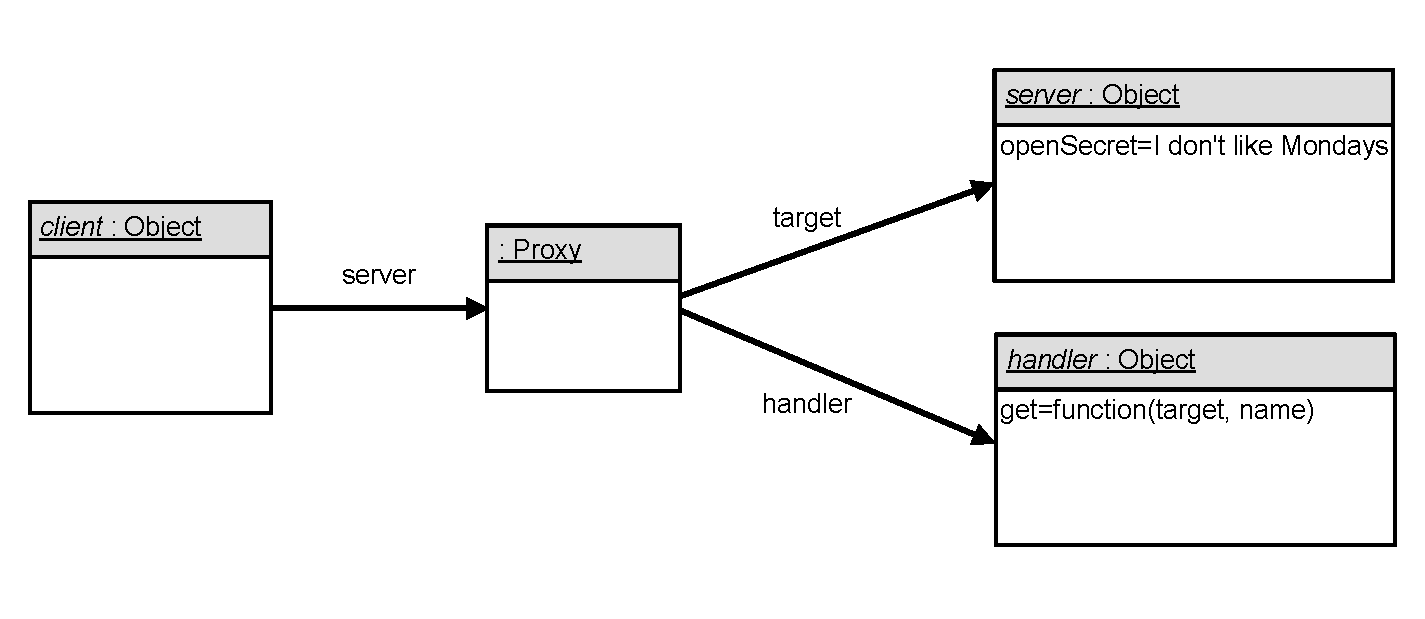
\includegraphics[width=\textwidth]{figures/5_implementation/1_loggingProxy.pdf}
    \caption{A \lstinline{client} object has access to a \lstinline{server} object via a proxy.}
    \label{fig:LoggingProxy}
\end{figure}

Listing~\ref{lst:loggingProxy} shows an example, in which a proxy is used to log property reads.
A \lstinline{client} object is connected to a \lstinline{server} object via a proxy, as shown in Figure~\ref{fig:LoggingProxy}:
The \lstinline{client}'s \lstinline{server} property is a reference to a proxy and that proxy's target is the \lstinline{server}.

\iffalse
\begin{verbatim}\fi
\begin{code}[lst:loggingProxy]{Using a proxy to log property reads to an object.}{float,numbers=left}
var client = {},
    server = {openSecret: "I don't like Mondays"},
    handler = {
        get: function(target, name) {
            console.log(name + ' was read at ' + Date());
            
            return target[name];
        }
    }

client.server = new Proxy(server, handler);
\end{code}
\iffalse
\end{verbatim}\fi

The proxy's \lstinline{handler} object implements a \lstinline{get} trap.
The \lstinline{get} trap receives two arguments when called: \lstinline{target} and \lstinline{name}.
The \lstinline{target} parameter refers to the proxy's \lstinline{target} object.
The \lstinline{name} parameter refers to the name of the property that was read.
In our example, the \lstinline{get} trap logs the property read (Line~5), then forwards the read to the \lstinline{target} object and returns the result (Line~7).
Therefore, reading a property of the server object via the proxy as shown in Listing~\ref{lst:propertyRead} would print a log statement similar to the following: ``openSecret was read at Sat May 10 2014 23:00:54 GMT+0200 (CEST)''.

\iffalse
\begin{verbatim}\fi
\begin{code}[lst:propertyRead]{Reading the \lstinline{openSecret} property of a \lstinline{client} object's \lstinline{server} property.}{float}
client.server.openSecret;
\end{code}
\iffalse
\end{verbatim}\fi

A handler object can implement traps for many different kinds of object interactions.
Table~\ref{table:traps} lists all possible traps with their parameters.

\begin{table}[h]
\begin{center}
\begin{tabular}{|l|l|r|}
\hline
get: function(target, name, receiver) \\ \hline
set: function(target, name, value, receiver) \\ \hline
apply: function(target, thisArg, args) \\ \hline
construct: function(target, args) \\ \hline
has: function(target, name) \\ \hline
hasOwn: function(target, name) \\ \hline
defineProperty: function(target, name, desc) \\ \hline
deleteProperty: function(target, name) \\ \hline
getOwnPropertyDescriptor: function(target,name) \\ \hline
getOwnPropertyNames: function(target) \\ \hline
getPrototypeOf: function(target) \\ \hline
freeze: function(target) \\ \hline
seal: function(target) \\ \hline
preventExtensions: function(target) \\ \hline
isFrozen: function(target) \\ \hline
isSealed: function(target) \\ \hline
isExtensible: function(target) \\ \hline
enumerate: function(target) \\ \hline
keys: function(target) \\ \hline
\end{tabular}
\caption[Table caption text]{Traps that proxy handlers can implement.}
\label{table:traps}
\end{center}
\end{table}

The traps fire either when a proxy is accessed with JavaScript operators or when it is passed to meta-programming facilities.
For example, the \lstinline{apply} trap fires when a proxied function is applied as shown in the following example:
\iffalse
\begin{verbatim}\fi
\begin{code}{}{}
proxy();
\end{code}
\iffalse
\end{verbatim}\fi
The \lstinline{preventExtensions} trap fires when a proxy is passed to the \lstinline{preventExtensions} function of the global \lstinline{Object}, which prevents subsequentely adding new properties to an object.
The trap would be triggered by statements such as the following:
\iffalse
\begin{verbatim}\fi
\begin{code}{}{}
Object.preventExtension(proxy);
\end{code}
\iffalse
\end{verbatim}\fi

When no trap is provided for a kind of object interactions, the proxy forwards the interaction transparently to the target.

The \lstinline{apply} trap and the \lstinline{construct} traps are only called, when a proxy's target is a function.

\paragraph{Using the Proxies as Virtual Objects}
The proxies require target objects to which they forward by default.
However, when a proxy's handler implements all traps, all intercepted interactions can be handled by the traps without forwarding to the target object.
Therefore, even though proxies have target objects, the target objects do not have to be accessed with any object interactions.
\\
This solution for using the proxies as virtual objects is also proposed by the official documentation\footnote{\url{http://wiki.ecmascript.org/doku.php?id=harmony:direct\_proxies\#virtual_objects}, accessed May 11, 2014}.



\subsection{Using the Proxies for Object Versioning} \label{subsec:IMPLEMENTATION:1.2}

The proxies stand in for multiple versions of an object in our implementation.
They forward all object interactions to a dynamically chosen version.

Figure~\ref{fig:VersioningProxy} exemplifies our usage of the proxies.
In the example, a proxy stands in for two versions of an \lstinline{address} object: The proxy's handler holds a reference to a \lstinline{versions} object, which in turn refers to the versions of the \lstinline{address} object.
The proxy's target is ommited from Figure~\ref{fig:VersioningProxy} as we used the proxies as virtual objects.
Therefore, they do not forward to their targets.

\begin{figure}[h]
    \centering
    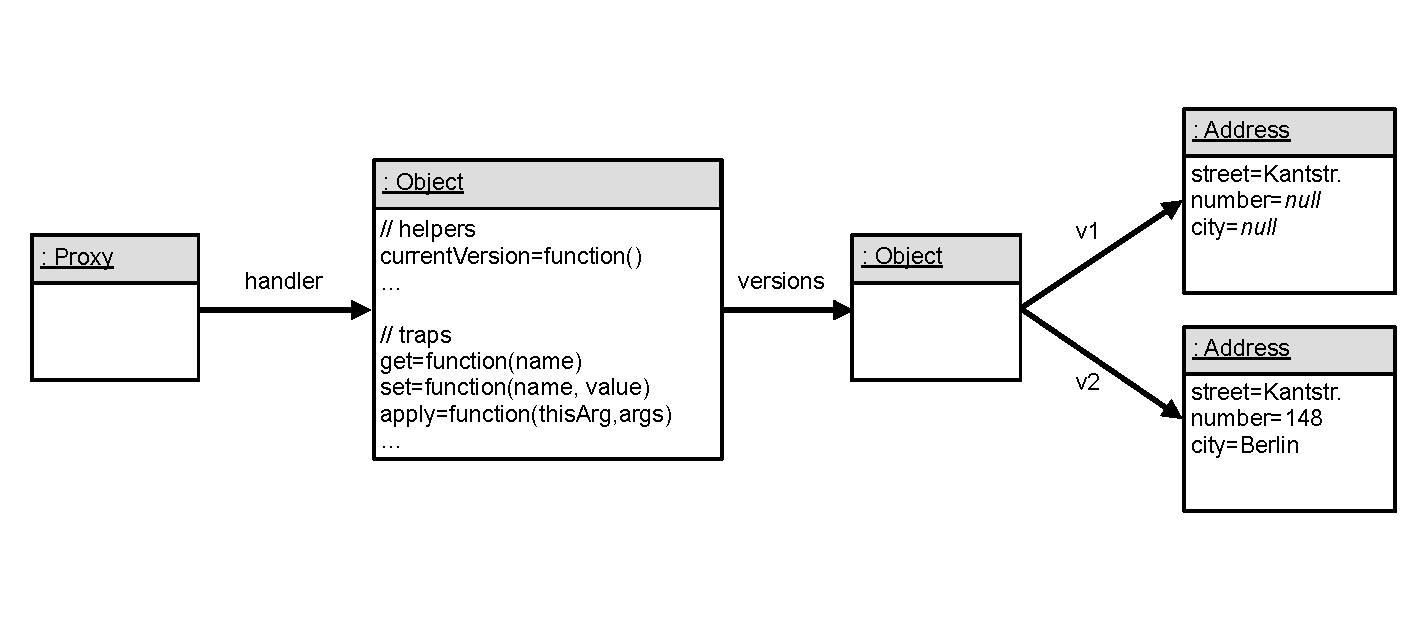
\includegraphics[width=\textwidth]{figures/5_implementation/2_versioningProxy.pdf}
    \caption{TODO}
    \label{fig:VersioningProxy}
\end{figure}

Our handler uses all traps to forward to the current version of an object.
For example, its \lstinline{get} trap works as shown in Listing~\ref{lst:getTrap}.

\iffalse
\begin{verbatim}\fi
\begin{code}[lst:getTrap]{TODO}{float,numbers=left}
get: function(dummyTarget, name) {
    var version = this.currentVersion();
    
    return version[name];
}
\end{code}
\iffalse
\end{verbatim}\fi

First, the trap retrieves the current version of the object using a helper function, which is named \lstinline{currentVersion} (Line~2).
Subsequentely, the trap reads the property from the current version and returns the result (Line~4).

The \lstinline{currentVersion} function chooses one of the versions of the object the proxy stands in for.
It does so according to the version of the system.
The version of the system is available globally as \lstinline{lively.CurrentVersion}.
It is an ordinary JavaScript object with three properties: an \lstinline{ID}, a \lstinline{predecessor}, and a \lstinline{successor}.
The \lstinline{currentVersion} function uses the \lstinline{ID} property to look up the correct version in its \lstinline{versions} object.

Object versions of previous system versions are not allowed to change.
However, when a version of an object is not changed in versions of the system, an object version of a previous system version reflects the current state.
Therefore, objects are not copied when they are not changed.
Instead, the \lstinline{currentVersion} function retrieves the latest available version as shown in Listing~\ref{lst:currentVersion}.

\iffalse
\begin{verbatim}\fi
\begin{code}[lst:currentVersion]{TODO}{float,numbers=left}
currentVersion: function() {
    var objectVersion,
        systemVersion = lively.CurrentVersion;
    
    while(!objectVersion && systemVersion) {
        objectVersion = this.versions[systemVersion.ID];

        systemVersion = systemVersion.previousVersion;
    }
    
    return objectVersion;
}
\end{code}
\iffalse
\end{verbatim}\fi

Traps that intercept changes are not allowed to forward to object versions of previous system versions.
Instead, they need to make sure that a version of the object exists for the current system version.
If such a version does not exist, the latest available version is copied and stored in the \lstinline{versions} object.

\begin{table}[h]
\begin{center}
\begin{tabular}{|l|l|r|}
\hline
set: function(target, name, value, receiver) \\ \hline
defineProperty: function(target, name, desc) \\ \hline
deleteProperty: function(target, name) \\ \hline
freeze: function(target) \\ \hline
seal: function(target) \\ \hline
preventExtensions: function(target) \\ \hline
apply: function(target, thisArg, args) \\ \hline
\end{tabular}
\caption[Table caption text]{Traps that intercept changes.}
\label{table:writeTraps}
\end{center}
\end{table}

% TODO: mutating interactions, mutating array functions

Listing~\ref{lst:versionForWriteAccess} shows the \lstinline{versionForWriteAccess} function that always returns an object version for the current system version.
The function is used by all traps that intercept changes, which are listed in Table~\ref{table:writeTraps}.
The \lstinline{apply} trap is included in this list, because built-in functions such as \lstinline{push} and \lstinline{pop} manipulate arrays.
The remaining traps select the version to forward using the \lstinline{currentVersion} function.

\iffalse
\begin{verbatim}\fi
\begin{code}[lst:versionForWriteAccess]{TODO}{float,numbers=left}
versionForWriteAccess: function() {
    var newVersion;
    
    if (!this.versions[lively.CurrentVersion.ID]) {
        newVersion = this.copyObject(this.currentVersion());
        
        this.versions[lively.CurrentVersion.ID] = newVersion;
    }
    
    return this.currentVersion();
},
\end{code}
\iffalse
\end{verbatim}\fi

Given the \lstinline{currentVersion} and the \lstinline{versionForWriteAccess} functions, the current version of the system is written as long as it is referred to by \lstinline{lively.CurrentVersion}.
To re-establish a different version, only this reference has to be changed.
Changing the global version is an undo, redo, or commit depending on whether the version is set to a previous, following, or new version.
For this, the system provides the functions \lstinline{lively.undo} (Listing~\ref{lst:undo}), \lstinline{lively.redo} (Listing~\ref{lst:redo}), and \lstinline{lively.commit} (Listing~\ref{lst:commit}).

\iffalse
\begin{verbatim}\fi
\begin{code}[lst:undo]{TODO}{float,numbers=left}
undo: function() {
    var predecessor = lively.CurrentVersion.predecessor;
    
    if (!predecessor) {
        throw new Error('Can\'t undo: No previous version.');
    }
    
    lively.CurrentVersion = predecessor;
}
\end{code}
\iffalse
\end{verbatim}\fi

\iffalse
\begin{verbatim}\fi
\begin{code}[lst:redo]{TODO}{float,numbers=left}
redo: function() {
    var successor = Lively.CurrentVersion.successor;
    
    if (!successor) {
        throw new Error('Can\'t redo: No next version.');
    }
    
    lively.CurrentVersion = successor;
}
\end{code}
\iffalse
\end{verbatim}\fi

\iffalse
\begin{verbatim}\fi
\begin{code}[lst:commit]{TODO}{float,numbers=left}
commit: function() {
    var predecessor = lively.CurrentVersion,
        newVersion;
    
    newVersion = {
        ID: predecessor.ID + 1,
        predecessor: predecessor,
        successor: null
    };
    predecessor.successor = newVersion;
    
    lively.CurrentVersion = newVersion;
}
\end{code}
\iffalse
\end{verbatim}\fi

Using a global version of the system is reasonable as JavaScript is executed single-threaded and scheduled cooperatively by the JavaScript engines.
While a script runs, the global version cannot be changed by another script.

 
\subsubsection{Scope of the Versioning} \label{subsubsec:IMPLEMENTATION:5.2.1}

Using the proxies allows for versioning JavaScript objects.
However, certain host objects cannot be versioned with our implementation.
These include the objects that represent the elements of the browser's \ac{dom}.
Some of \ac{dom} objects cannot be copied.
For this reason, it is not possible to create multiple versions of them.
Moreover, the \ac{dom} objects are referred to from the browser's \ac{dom}, which is external to the JavaScript runtime and which, thus, does not use version-aware references.
However, this is not a problem, because the state of the \ac{dom} can be derived from the Lively Kernel's morph objects.
Therefore, we update the \ac{dom} from the current set of visible morphs when the system version changes.
Besides these host objects, all objects that are accessed through our proxies are versioned with the system versions.





\section{Proxies For All Mutable JavaScript Objects}

To be able to re-establish the entire state with our versioning, our proxies need to be used to access all objects, arrays, and functions.
This is necessary because objects, arrays, and functions are mutable in JavaScript.
In fact, functions and arrays are objects.
They can have arbitrary properties.

Our implementation changes the return values of all expressions that create new objects.
Instead of letting these expressions return references to the new objects, the expressions return references to proxies for the objects.
As a result, references to proxies are passed around instead of references to objects so that all access goes through the proxies.

In JavaScript, there are three categories of expressions that create new objects: 
\begin{itemize}
    \item literal expressions: e.g. \lstinline|{age: 12}|
    \item constructor functions: e.g. \lstinline|new Person(12)|
    \item specific built-in functions: e.g. \lstinline|Object.create(prototype, {age: 12})|
\end{itemize}

Our implementation uses source transformations and proxy traps to have these expression return proxies.


\subsection{Transforming Literal Expressions}

We use source transformations to wrap literal expressions into calls to a \lstinline{proxyFor} function.
The \lstinline{proxyFor} function returns a proxy for its argument.
The transformations for literal objects, arrays, and functions are shown in Table~\ref{table:literalTransforms}.

\begin{table}[h]
\begin{center}
\begin{tabular}{| l | l | l |}
\hline
Type & Input & Output \\ \hline
\emph{Objects} & \lstinline|{name: 'James', age: 24}| & \lstinline|proxyFor(name: 'James', age: 24)| \\ \hline
\emph{Arrays} & \lstinline|[person1, person2]| & \lstinline|proxyFor([person1, person2])| \\ \hline
\emph{Functions} & \lstinline|function (a, b) {..}| & \lstinline|proxyFor(function (a, b) {..})| \\ \hline
\end{tabular}
\end{center}
\caption[Table caption text]{Transforming literal objects, arrays, and functions.}
\label{table:literalTransforms}
\end{table}

However, some literal forms cannot be wrapped into function calls without introducing problems.
In particular, function declarations and accessor functions need to be handled differently.


\subsubsection{Function Declarations}

A \emph{function declaration} is a function literal that creates a named function and makes it available by the name.
It does not need to be assigned to a variable to be available in the surrounding scope.
The following statement is a function declaration:
\iffalse
\begin{verbatim}\fi
\begin{code}{}{}
function add(a, b) {return a + b}
\end{code}
\iffalse
\end{verbatim}\fi

In contrast, a \emph{function expression} creates a function that needs to be assigned to a variable to be accessible.
The following statement assigns a function expression to a variable:
\iffalse
\begin{verbatim}\fi
\begin{code}{}{}
var subtract = function(a, b) {return a - b}
\end{code}
\iffalse
\end{verbatim}\fi

Function expressions can create anonymous and named functions.
The example above creates an anonymous function.
The following example assigns a named function to a variable:
\iffalse
\begin{verbatim}\fi
\begin{code}{}{}
var multiply = function multiply(a, b) {return a * b}
\end{code}
\iffalse
\end{verbatim}\fi

An anonymous function is always a function expression.
A named function is either a function expression or a function declaration, depending on where it is expressed.
A function declaration cannot be nested into other statements such as variable assignments.
It has to start with the \lstinline{function} keyword.

Therefore, when a function declaration is wrapped into a function call, it becomes a function expression.
The function would no longer be available by its name in the surrounding scope.
For this reason, the function declarations that are wrapped into calls to the \lstinline{proxyFor} function are assigned to matching variable names.
Table~\ref{table:funcTransform} shows an example for this transformation.

\begin{table}[h]
\begin{center}
\begin{tabular}{| l | l | l |}
\hline
Input & Output \\ \hline
\lstinline|function div() {}| & \lstinline|var div = proxyFor(function div() {})| \\ \hline
\end{tabular}
\end{center}
\caption[Table caption text]{Transforming a function declaration.}
\label{table:funcTransform}
\end{table}

In addition, because function declarations get hoisted in JavaScript, transformed function declarations are moved to the beginning of the defining scope.


\subsubsection{Accessor Functions}

Accessor functions are functions that are executed transparently instead of property reads or writes.
Listing~\ref{lst:accessorOriginal} shows an example in which an accessor function is used to allow reading a \lstinline{person}'s \lstinline{age} even though the \lstinline{person} object only has a \lstinline{birthdate} property.

\iffalse
\begin{verbatim}\fi
\begin{code}[lst:accessorOriginal]{TODO}{float,numbers=left}
var person = {
    birthdate: new Date(1984,27,5),
    get age() {
        return ageToday(this.birthdate);
    }
}
\end{code}
\iffalse
\end{verbatim}\fi

Wrapping the accessor function into the \lstinline{proxyFor} function would not yield valid JavaScript syntax.
However, accessor functions can also be defined with the \lstinline{Object.defineProperty} function.
Therefore, the object is created without accessor functions and the accessor function defined separately using \lstinline{Object.defineProperty}.
Both the object and the accessor functions can be wrapped into calls to the \lstinline{proxyFor} function when expressed in this way.
Listing~\ref{lst:accessorTransformed} shows the result of transforming the example in Listing~\ref{lst:accessorOriginal}.
The new object is created in an anonymous functions that is applied directly.
In this anonymous function, the new object is assigned to a variable called \lstinline{newObject}.
This allows to have the object be available in a variable for the subsequent \lstinline{Object.defineProperty}-function call without polluting the variable bindings of the originally surrounding scope.

\iffalse
\begin{verbatim}\fi
\begin{code}[lst:accessorTransformed]{TODO}{float,numbers=left}
var person = function() {
    var newObject = lively.proxyFor({
        birthdate: new Date(1984,27,5);
    });
    Object.defineProperty(newObject, "age", {
        get: lively.proxyFor(function age() {
            return ageToday(this.birthdate);
        })
        enumerable: true,
        configurable: true
    });
    return newObject;
}();
\end{code}
\iffalse
\end{verbatim}\fi



\subsection{Returning Proxies from Constructor Functions} 

When functions are used as constructors, they need to return proxies.
In JavaScript, all functions can be used as constructors and create objects when called with the \lstinline{new} operator.
Listing~\ref{lst:constructorFunction} shows how a literal function is used to construct a new object.

\iffalse
\begin{verbatim}\fi
\begin{code}[lst:constructorFunction]{TODO}{float, numbers=left}
function Person() {}
var someone = new Person();
\end{code}
\iffalse
\end{verbatim}\fi

We use the \lstinline{construct} trap to return proxies from proxied functions used as constructors.
Listing~\ref{lst:constructTrap} shows the \lstinline{construct} trap of our proxy handlers.

\iffalse
\begin{verbatim}\fi
\begin{code}[lst:constructTrap]{TODO}{float,numbers=left}
construct: function(dummyTarget, args) {
    var constructor, prototype, newObject, result;
    
    constructor = this.currentVersion()
    
    prototype = constructor.prototype ? constructor.prototype : {}    
    newObject = Object.create(prototype);
    
    result = constructor.apply(newObject, args);
    
    return proxyFor(result ? result : newObject);
}
\end{code}
\iffalse
\end{verbatim}\fi

The \lstinline{construct} trap does the following:
\begin{enumerate}
    \item It retrieves the current version of the constructor (Line~4).
    \item It creates a new object with the correct prototype (Line~7).
    \item It applies the constructor to the new object (Line~9).
    \item It returns a proxy for either the return value of the constructor function or, in case the constructor did not return a value, the new object (Line~11).
\end{enumerate}

This way, all proxied functions return proxies when used as constructors.
With the transformations of literal functions presented in the previous subsection all literal functions are accessed through proxies.
However, there are also functions built into the JavaScript engines.
These are not created from function literals and, therefore, cannot be proxied by transforming literals.


\subsection{Wrapping Built-in Functions}

Some built-in functions can be used to create new objects.

For example, objects and arrays can be created by evaluating \lstinline{new Object()} and \lstinline{new Array()}.
% can also be called without the new operator: Object() / Array()
% Object.create()
% eval()


% OBJECT() / ARRAY .. 

We transform built-in constructor functions explicity, wrapping each into calls to the \lstinline{proxyFor} function.

% example:      Object() --> proxyFor(Object)()

% returns a proxy for the function object \lstinline{Object}.. 
% \lstinline{construct} trap:  for functions then return proxies for the newly created objects from their construct-traps.

% This is also true for the \emph{apply} trap, because, for example, the \lstinline{Array} and \lstinline{Object} functions also create objects when called without the \lstinline{new} operator and, for example, the built-in function \lstinline{Object.create(proto)} also returns a new object.



% OBJECT.CREATE

% object.create.. wrapping object.. 

% example:      Object.create(proto) --> proxyFor(Object).create(proto)

% the \emph{get}-trap also makes sure to return always proxy in this fashion.


% this way. it is enough to wrap Object into proxyFor.. to have Object.create be proxied as well, even though the actual \lstinline{Object} object does not refer to its \lstinline{create} function through a proxy.
% So, wrapping \lstinline{Object} is enough to have \lstinline{Object.create(proto)} return a proxy: \lstinline{Object.create(proto)} transforms to \lstinline{proxyFor(Object).create(proto)} and getting the property \emph{create} then returns a proxy for the function, which when applied also returns a proxy.

% therefore, the source transformations wrap the global objects, but do not wrap each of the properties.




% EVAL

there are also very specific built-in functions, that we transform separately to specific alternatives.
One example for such a function is the global \lstinline{eval} function.
\lstinline{eval} takes arbitrary code which might express an arbitrary object structure and which, therefore, might require proxies for multiple objects.
In the specific case of eval, we proxy \lstinline{eval}'s result but additionally also pass its string argument through the source transformations.



% PROXY TABLE

For example, \lstinline{Array(100)} becomes \lstinline{proxyFor(Array(100))}.
As every call to such built-in objects is transformed in this way, the same Object---in this case the \lstinline{Array} function---gets passed to the \lstinline{proxyFor} function multiple times.
To nevertheless return the same proxy, we use a map that associates objects with their proxies.
This \emph{Proxy Table} is a weak-key map and does prevent the version objects used as keys from being gargabe collected when their proxies get garbage collected.
Using the same proxies for objects is also necessary for identity checks.
That is, the following statement yields true for an arbitrary object \lstinline{obj}: \lstinline{proxyFor(obj) === proxyFor(obj)}.




% SOURCE TRANSFORMATION, NO MONKEY PATCHING

% The built-in functions could be overwritten globally to return proxies for the new objects, but our implementation of object versioning is itself just a JavaScript library and makes itself use of the built-in data types.
% Additionally, at the time of writing, some JavaScript engines do not allow to overwrite particular built-in functions and we want our implementation of object versioning to work in every JavaScript engine that supports the ECMAScript 6 Direct Proxies.













\subsubsection{Implementation of Source Transformations}

Our implementation uses \emph{UglifyJS}\footnote{\url{http://github.com/mishoo/UglifyJS2}, accessed March 12, 2014} for all source transformations.
UglifyJS parses source code without relying on JavaScript exceptions.
Therefore, when code is transformed before evaluation and the transformation steps do not yield exceptions that could be caught by an open debugger.
In addition, UglifyJS supports Source Maps \footnote{\url{https://docs.google.com/document/d/1U1RGAehQwRypUTovF1KRlpiOFze0b-_2gc6fAH0KY0k/edit\#heading=h.ue4jskhddao6}, accessed May 2, 2014}.
This way, the browser's developer tools, including the debugger, present the original sources, even though transformed code is executed.

% rough sketch of how transformations are done???
    % code of modules passed to source transformation. parsing, AST transformations, printing. 








\section{Workarounds for the Current State of the Proxies} \label{sec:IMPLEMENTATION:4}

% TODO: each subsection should be divided into a problem and a solution/approach/workaround part/subsubsection

Certain workarounds are required due to the preliminary status of the proxy implementation.

While the specification of Direct Proxies already progressed from proposal status to being part of the current ECMAScript 6 Draft\footnote{\url{http://people.mozilla.org/~jorendorff/es6-draft.html}, accessed March 5th, 2014}, it is still in draft status and not yet implemented in the JavaScript engines used by Chrome and Firefox.
These two engines currently both implement two different deprecated proposals for the proxies instead of the most recent ECMAScript 6 Draft.
The \emph{harmony-reflect} library\footnote{\url{http://github.com/tvcutsem/harmony-reflect}, accessed February 3, 2014, used version 0.0.11}, however, provides the current API of Direct Proxies for recent versions of both Chrome and Firefox, on top of the implementations of the different deprecated proposal states.
That is, our implementation uses the \emph{harmony-reflect} shim and, thereby, works in both Chrome and Firefox.

However, even with the shim, three issues need to be addressed with technical workarounds:

\begin{enumerate}
    \item The proxies have to be provided with an actual target, even when implementing virtual objects, and consistency invariants compare return values of traps to the state of the actual target. 
    \item The proxies do not intercept the \lstinline{instanceof} operator, but always delegate to the current target.
    \item Certain built-in JavaScript functions dont handle proxies correctly.
\end{enumerate}

These workarounds might no longer be necessary once the ECMAScript 6 standard gets finalized and fully implemented by the JavaScript engines. 


\subsection{Disabling Target Object Invariants}

% While these are supposed to stand in for particular objects, their \emph{targets}, they can also be used as fully virtual objects.

Using the \emph{harmony-reflect} shim in a recent Chrome, proxies require an actual \emph{target} object even though the current ECMAScript 6 draft says otherwise\footnote{\url{http://people.mozilla.org/~jorendorff/es6-draft.html\#sec-proxy-object-internal-methods-and-internal-slots}, accessed April 15, 2014}.

When an actual target object is provided on creation of a proxy, the internal link between proxy and target object is fixed and cannot be changed at runtime.
Therefore, in our use case of the proxies, in which proxies stand in for a group of objects from which one is chosen dynamically, the proxy is still linked to a particular object by default.
Additionally, the Direct Proxies are designed to ensure invariants between the trap behavior and the target's properties~\cite{Cutsem2013TRP}.

For example, when an object's properties are made immutable using \lstinline{Object.freeze}, the invariants ensure that the target object has in-fact been frozen, even if the trap delegates the operation to another object such as one of our versions of an object.
Further, another invariant ensures that all immutable values of the target object are returned correctly by the \lstinline{get}-trap, even when the \emph{get}-trap reads from another object than the target. 
That is, in our case, configuring any property as immutable would effectively declare make that property immutable for all versions.
Additionally, in this scenario, reading the property in a version where the value of this property is different from what it is in the immutable target would raise incosistency errors.

For this reason, we adapted our copy of the \emph{harmony-reflect} library.
In particular, we added a boolean flag to the Proxy constructor function that indicates whether a proxy is standing in for one target object or is a virtual object.
This boolean flag is then used to disable all consistency checks when a proxy is meant to be a virtual object.

The proxy constructor still requires an actual object as \emph{target} object, but this target object is now only used for the \lstinline{typeof} operator for the virtual object-kind of proxies.

The \lstinline{typeof} operator returns only a distinction between a certain set of types in JavaScript.
The only necessary difference for the \lstinline{typeof} operator is that a proxy representing the versions of an object or array has an object as target, while a proxy representing the versions of a function needs to have a function as target.
This difference in the type of supplied target objects is also necessary as the \emph{apply}- and \emph{construct}-trap are also only called on proxies with functions as targets.


\subsection{Forwarding the \emph{Instanceof} Operator}

There is currently no \lstinline{instanceof} trap to intercept the behavior of the \lstinline{instanceof} operator.

The \lstinline{instanceof} operator returns the of an object, which is defined by an object's prototype chain in JavaScript.
The prototype of an object is a property and can be changed at runtime.
It gets versioned as any other property.
The \lstinline{instanceof} operator, thus, also needs to be delegated to the current version of an object.
% When creating a proxy a \emph{target} object can be provided to be linked from the proxy and the \lstinline{instanceof} operator would follow this link to report the target's type, but as the target link cannot be changed later on, while proxies stand in for multiple versions with potentially different types, this is not an option.

For this, we implemented a custom \lstinline{Object.instanceof} function, which implements the semantics of the \lstinline{instanceof} operator but does delegate to the correct version of an object.
All usage of the \lstinline{instanceof} operator is then transformed to usage of the custom function.
These transformations change code as shown by the following example: 

% TODO: table!

\iffalse
\begin{verbatim}\fi
\begin{code}[]{}{float}
anObject instanceof Type -> Object.instanceof(anObject, Type)
\end{code}
\iffalse
\end{verbatim}\fi

While there is no trap for the \lstinline{instanceof} operator in the current specification, trapping the operator is under discussion\footnote{\url{http://wiki.ecmascript.org/doku.php?id=harmony:direct_proxies\#discussed_during_tc39_july_2012_meeting_microsoft_redmond}, accessed May 1, 2014}.


\subsection{Unwrapping Versions for Native Code} \label{subsec:IMPLEMENTATION:4.3}

Some built-in JavaScript functions react to proxies with actual errors, return wrong results, or otherwise do not provide the usual functionality.
Therefore, these functions need to be provided with actual objects instead of the proxy.
% This is unproblematic for most cases as, given JavaScript's single-threaded and cooperative execution in browser engines, which version of an object is to be used is not expected to change during the execution of a built-in function.
Our implementation provides the current version of an object to these built-in functions through proxy handler traps and patched built-in functions.

The \emph{apply}-trap, called when proxied functions get applied, unwraps all arguments and the \emph{thisContext} object, when the applied function is a built-in functions that does not handle proxies correctly.
This is for example the case for the functions that provide access to the browser's \ac{dom}.

The \emph{set}-trap sometimes needs to unwrap the assigned value when that value is proxied and gets assigned to slots that cannot handle proxies.
This is for example the case with the \lstinline{onreadystatechange} slot of \emph{XMLHttpRequest} objects.
This particular slot holds functions as callbacks of asynchronous HTTP requests, which, however, do not get called when these functions are proxies.

Unwrapping a particular version from a proxy for an asynchronous callback is potentially problematic.
Though JavaScript does get executed with a single thread using cooperative scheduling by all popular browsers, other concurrent scripts might get executed and switch the global version before the callback can be called.
It is, however, unlikely that a callback function's \emph{properties} are changed while waiting for the response and even bad programming style as it introduces dependencies on network timing even without proxies.
Therefore, our implementation currently does not provide a workaround for this specific case, even though we are aware of this potential problem. 

In addition to unwrapping in traps, there are also certain immutable types that do not get proxied at all in our implemention such as strings.
Strings, however, do have methods and these also do not handle proxies correctly.
As the arguments to these methods is not handled in traps, because strings are not proxied, our implementation patches such functions with functions that unwrap proxies before executing the original functions.


% TODO: get-trap.. proxy X to proxy X.method()..

% TODO: code?




\section{Limitations of the Implementation}

The current implementation has three limitations.

\paragraph{Availability of ECMAScript 6 Proxies}
Our implementation requires the ECMAScript 6 Direct Proxies to be available.
The proxies are, however, part of the next version of ECMAScript, which has currently neither been finalized nor completely implemented, as described in \ref{sec:IMPLEMENTATION:4}.
For this reason, our implementation works only in recent versions of Firefox and Chrome that already implement preliminary versions of the proxies.
For Chrome, users also need to enable the proxies through explicitly setting the \emph{Experimental JavaScript}-option.

\paragraph{Proxies Impede Developer Tools}
The current implementation of proxies impedes debugging.
The proxies are partly implemented by a JavaScript library and every trapped object access is visible in multiple frames in the debugger.
That is, the stack of the debugger is cluttered with frames that belong to the proxy implementation, not to the application source code.
In addition, the developer tools in Chrome do not handle proxies correctly under all circumstances.
In particular, hovering variable names that are currently bound to proxies yields errors and stepping into proxied functions does not work.

\paragraph{Concurrent JavaScript}
Even though JavaScript is executed with a single thread, scripts can be executed concurrently.
In general, scripts can be started from events and explicitly from other scripts using the \lstinline{setTimeout} or the \lstinline{setInterval} function.
Switching the system version can be problematic for such concurrently running scripts.
For example, the Lively Kernel makes use of the \lstinline{setInterval} function to repeatedly execute a method of an object.
Re-establishing a previous version can interfere with such ticking behavior as the object or its method can be unavailable in previous versions.
For this reason, we stop scripts from future versions, when the system version changes.
We did, however, not succeed in finding a way to restart the scripts again when the future versions are re-established.
Thus, subsequentely undoing and redoing changes can stop concurrently running scripts.

% single-threaded and cooperative scheduling, but setTimeout / setInterval... stop asynchronous actions from following versions when undoing... source transformations, which scripts belongs to which version
